\section{Constraint-Programmierung}
\subsection{Constraints}
Ein Constraint (engl. \textsl{to constrain} - dt. \textsl{einschränken}) ist 
eine logische Formel, welche die möglichen Werte einer Variablen beschränkt 
\cite{KI-LP96}. In Oz gibt es mehrere Constrainttypen. Elementare Constraints 
sind Gleichungen zwischen Variablen bzw. zwischen einer Variablen und einer 
Struktur. Listing \ref{lst:elementare-constraints} zeigt einige Beispiele für 
elementare Constraints.

\begin{lstlisting}[
caption={Beispiele für elementare Constraints}, 
label={lst:elementare-constraints}]
X = 23
X = Y
X = pair(Y Z)
X = student(matrikel:M semester:S name:N)
\end{lstlisting}

Neben diesen elementaren Constraints lassen sich in Oz auch sog. \textsl{finite 
domain constraints} verwenden. Mit diesen können Variablen auf endliche 
Intervalle ganzer Zahlen beschränkt werden. Beispielsweise schränkt 
\lstinline{X :: 1#42} die Variable $X$ auf ganze Zahlen zwischen 1 und 42 ein,
also $X \in (1, 42)$.

\subsection{Constraintbasierte Problemlösung}
Es existiert eine Reihe kombinatorischer Probleme, die sich mit Variablen 
ausdrücken lassen, die ganzzahlige, nichtnegative Werte in einem 
abgeschlossenen Intervall annehmen. Um diese Art von Problemen mithilfe von Oz 
zu lösen, lassen sich die vorgestellten finite domain constraints verwenden.

Einige Beispiele für solche Probleme sind:

\begin{description}
  \item[$N$ Damen.] Auf einem Schachbrett sollen $N$ Damen so platziert werden, 
  dass sie sich gegenseitig nicht schlagen können.
  \item[Kartenfärbung.] Eine Landkarte (oder allgemein ein Graph) soll so 
  eingefärbt werden, dass benachbarte Länder unterschiedliche Farben haben und 
  die Anzahl der verwendeten Farben minimal ist.
  \item[Send More Money.] Gegeben sei die Gleichung $SEND + MORE = MONEY$. Nun 
  soll den einzelnen Buchstaben jeweils eine Ziffer zwischen 0 und 9 zugewiesen 
  werden, sodass die Gleichung erfüllt ist. Weiterhin soll $S \neq 0$ sowie $M 
  \neq 0$ gelten.
\end{description}

Konkret werden diese Probleme mithilfe zweier Techniken gelöst, die wir im
folgenden vorstellen möchten.

\subsubsection{Propagierung}
Der Constraintspeicher enthält lediglich die zuvor eingeführten "`einfachen"' 
Constraints. Zur Lösung kombinatorischer Probleme werden aber u.U. komplexere 
Constraints, wie z.B. arithmetische Gleichungen benötigt. Hier kommen die sog. 
Propagierer ins Spiel. Ein Propagierer hat eine deklarative Semantik; bei 
dessen Reduktion werden diejenigen "`einfachen"' Constraints im 
Constraintspeicher explizit gemacht, die durch die Semantik des Propagierers 
impliziert werden. Beispiele für Propagierer sind in Listing 
\ref{lst:propagierer} aufgeführt.

\begin{lstlisting}[caption={Beispiele für Propagierer}, label={lst:propagierer}]
X < Y
X^2 + Y^2 = Z^2
5X - 3Y > 2Z
\end{lstlisting}

\paragraph{Beispiel} Gegeben sei ein Constraintspeicher mit dem folgenden 
Inhalt: $$X \in 0\#9 \, \wedge \, Y \in 0\#9$$ sowie zwei Propagatoren: $$P_1: 
X + Y = 9, \qquad P_2: 2X + 4Y = 24$$ Die Propagierung läuft nun folgendermaßen 
ab:

\begin{enumerate}
  \item $P_1$ liefert keine neuen Erkenntnisse, $P_2$ hingegen kann aufgrund der
  im Constraintstore vorhandenen Information die Wertebereiche für $X$ und $Y$
  einschränken: $X \in 0\#8$ und $Y \in 2\#6$.
  \item $P_1$ kann nun $X$ einschränken: $X \in 3\#7$; $Y$ bleibt unverändert. 
  \item $P_2$ schränkt weiter ein: $X \in 4\#6$ und $Y \in 3\#4$.
  \item $P_1$ wird erneut aktiviert und es ergibt sich: $X \in 5\#6$ und $Y \in
  3\#4$.
  \item Schließlich folgert $P_2$: $X = 6$ und $Y = 3$. Damit sind die Werte der
  Variablen eindeutig bestimmt. \cite[Finite Domain Constraint Programming in
  Oz, Chapter 2.3]{url:mozart-documentation}
\end{enumerate}

Die Propagierung stellt ein deterministisches Verfahren dar, welches allerdings 
nicht unbedingt vollständig ist. Das bedeutet, dass u.U. sowohl existierende 
Lösungen nicht gefunden werden, als auch die Nichtexistenz von Lösungen nicht 
erkannt wird \cite{KI-LP96}.

\subsubsection{Distribuierung}
Um ein vollständiges Lösungsverfahren zu erhalten, muss zusätzlich die sog.
Distribuierung eingesetzt werden. Dabei wird das Problem in Unterprobleme
aufgeteilt; es entsteht ein Suchbaum, der beispielsweise auch verteilt
durchsucht werden kann.

Sobald ein Problem $P$ nicht mehr durch Propagierung gelöst werden kann, wird 
$P$ so in $P_1$ und $P_2$ aufgeteilt, dass gilt: $P = P_1 \wedge P_2$. Diese 
Aufteilung nennt man Distribuierung. Es wird nun versucht, die beiden 
Teilprobleme in separaten Berechnungsräumen zu lösen. Dazu kann man oftmals 
einfach einen neuen Constraint $C$ wählen, dessen Negation $\neg C$ ebenfalls 
einen Constraint darstellt, und mit diesen neuen Propagatoren in den beiden 
Zweigen des Baumes die Propagierung fortsetzen. Wann immer die Propagierung 
nicht weiterhilft, wird der Baum nach diesem Schema weiter aufgeteilt.

\paragraph{Beispiel} Gegeben sei ein Constraintspeicher mit dem folgenden
Inhalt: $$X \in 1\#3 \, \wedge \, Y \in 2\#3 \, \wedge \, Z \in 1\#4$$ sowie
zwei Propagatoren: $$P_1: X < Y, \qquad P_2: X^2 = Z$$
Nun läuft zunächst die Propagierung ab:

\begin{enumerate}
  \item $P_1$ schränkt ein: $X \in 1\#2$.
  \item $P_2$ wird aktiv und schränkt ein: $Z \in 1\#4$.
\end{enumerate}

Zu diesem Zeitpunkt bringt die Propagierung keine weiteren Erkenntnisse, es ist 
aber auch noch keine Lösung bestimmt worden. Durch Kopieren des 
Berechnungsraums wird nun der Suchbaum erstellt und im linken Teilbaum mit $C: 
X = 1$, im rechten mit $\neg C: X \neq 1$ weiter propagiert. Man erhält den in 
Abbildung \ref{fig:distribuierung-suchbaum} dargestellten Suchbaum - es ergeben 
sich schließlich drei Lösungen, markiert durch die grünen Rauten in 
\ref{fig:distribuierung-suchbaum-2}.

\begin{figure}
  \centering \subfloat[Suchbaum mit Werten]{
    \label{fig:distribuierung-suchbaum-1}
  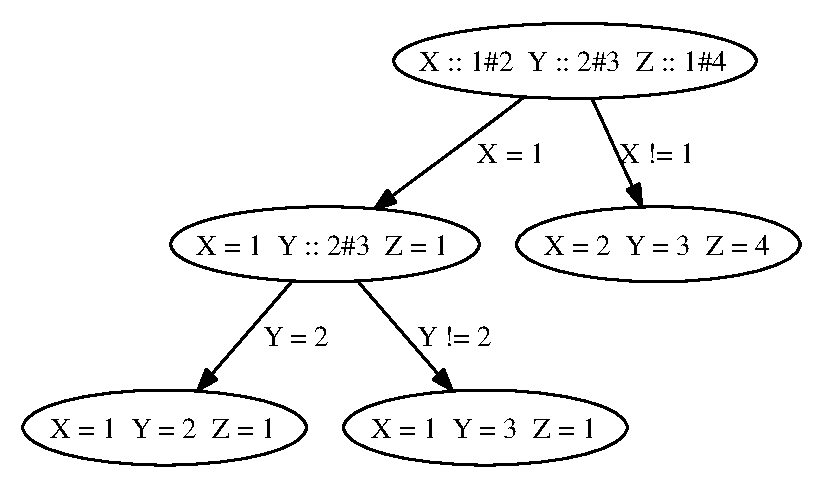
\includegraphics[height=6cm]{../images/searchtree-values} 
  } \subfloat[Suchbaum als Graph]{
    \label{fig:distribuierung-suchbaum-2}
  \includegraphics[height=6cm]{../images/searchtree-graph} 
  }
  \caption{Distribuierung}
  \label{fig:distribuierung-suchbaum}
\end{figure}

\subsection{Beispiel "`Send More Money"'}
Nachfolgend möchten wir anhand eines konkreten Beispiels die 
Wissensverarbeitung mithilfe der Constraint Programmierung in Oz demonstrieren. 
Entnommen ist diese Lösung des "`Send More Money"'-Problems der 
Mozart-Dokumentation \cite[Finite Domain Constraint Programming in
  Oz, Chapter 3.2]{url:mozart-documentation}.

\subsubsection{Problemdefinition und Modell}
Gegeben sei die Gleichung $$SEND + MORE = MONEY$$ Ziel ist es, den einzelnen
Buchstaben paarweise verschiedene Ziffern zwischen 0 und 9 zuzuweisen. Außerdem
soll gelten: $S \neq 0$ und $M \neq 0$.

\subsubsection{Programm}
Listing \ref{lst:sendMoreMoney} zeigt den Quellcode des fertigen Oz-Scripts.

\lstinputlisting[label={lst:sendMoreMoney}, caption={Das "`Send More 
Money"'-Problem in Oz}]{../sendMoreMoney.oz}

Es werden zunächst für alle Buchstaben Variablen deklariert und anschließend ein
\texttt{Record} angelegt, der für jeden Buchstaben einen Eintrag enthält (Zeile
6). In den nachfolgenden Zeilen werden die einzelnen Constraints deklariert: 

\begin{itemize}
  \item alle Einträge in \texttt{Root} sind beschränkt auf $(0, 9)$,
  \item alle Einträge in \texttt{Root} sind paarweise verschieden (distinct),
  \item S und M sind ungleich 0,
  \item die Werte der einzelnen Buchstaben erfüllen die Gleichung.
\end{itemize}

In Zeile 14 wird die Distribuierung mit der sog. "`first-fail"'-Strategie 
angestoßen. Bei dieser Strategie wird zur Erzeugung des zur Distribuierung
benötigten Constraints die höchstwertige Variable verwendet, bei der die Anzahl
möglicher Werte minimal ist.

Schließlich wird in Zeile 17 die Suche nach der Lösung begonnen (s. Kapitel 
\ref{subsection:Search}) und in der darauf folgenden Zeile der Suchbaum 
ausgegeben.

\subsection{Beispiel Sudoku}
Anhand eines weiteren Beispiels möchten wir die Lösung von Problemen und die 
Wissensverarbeitung in Oz zeigen. Sudoku ist ein Logikrätsel, das sich in den 
letzten Jahren großer Beliebtheit erfreut hat. In der Regel besteht ein 
Sudoku-Rätsel aus einem $9 \times 9$-Gitter, das mit einigen Zahlen vorbelegt 
ist. Ziel ist es, die freien Felder des Gitters so zu füllen, dass in der jeder 
\textsl{Reihen}, \textsl{Spalten} und in jedem der neun \textsl{$3 \times 
3$-Unterquadrate} die Ziffern zwischen 1 und 9 genau einmal vorkommen.

Abbildung \ref{fig:sudoku-beispiel} zeigt ein Beispiel für ein Sudoku-Rätsel im
Startzustand.

\begin{figure}[hp]
	\begin{sudoku}
	| |1|2| | |9|6| | |.
	| | |7|3|5| | |9| |.
	|8| | | |4| | |3|7|.
	|4| |3|2| | | |1| |.
	| |8| |7|6| |9| | |.
	|9| | | | |3|8| |4|.
	| |6| | | |5|7| |1|.
	|7| |9|6| |1| | | |.
	| |5| | |2| | |6|9|.
	\end{sudoku}
  \caption{Ein $9 \times 9$-Sudoku}
  \label{fig:sudoku-beispiel}
\end{figure}

\subsubsection{Problemdefinition und Modell}

Gegeben sei ein Sudoku Quadrat der Ordnung $n$, das ein $n^2 \times n^2$-Gitter 
mit $n^4$ Felder mit den Werten von $0$ bis $n^2$ bildet 
\cite{sudoku-as-constraint}. Jeder Wert, $0$ bis $n^2$, darf in jeder Reihe, 
jeder Spalte und in jedem der $n^2$ $n \times n$-Unterquadrate genau einmal 
vorkommen.

Üblicherweise werden Sudokus der Ordnung $3$ ($9 \times 9$-Gitter) verwendet.
Laut \cite{sudoku-as-constraint} gibt es 6.670.903.752.021.072.936.960 komplett
ausgefüllte und gültige Sudoku-Quadrate der Ordnung $3$.


Darstellen lässt sich das Sudoku-Problem (hier: $9 \times 9$-Sudoku) auch als
Graphfärbeproblem, wie Abbildung \ref{fig:sudoku-graph} zeigt.

\begin{figure}
  \centering
  \def\JPicScale{0.5}
  \input{../images/sudoku-graph.pst}
  \caption{Linker oberer Block eines Sudoku-Rätsels als Graph}
  \label{fig:sudoku-graph}
\end{figure}

Aus diesem Graphen lässt sich direkt ableiten, wann ein Knoten mit einem anderen
Knoten durch eine Kante verbunden ist. Dies ist genau dann der Fall, wenn

\begin{itemize}
  \item $x = x'$, (Knoten liegen in derselben \textsl{Spalte}) oder
  \item $y = y'$, (Knoten liegen in derselben \textsl{Zeile}) oder
  \item $\left\lceil \nicefrac{x}{3} \right\rceil = \left\lceil
  \nicefrac{x'}{3} \right\rceil \wedge \left\lceil \nicefrac{y}{3} \right\rceil
  = \left\lceil \nicefrac{y'}{3} \right\rceil$ (Knoten liegen im selben
  $3 \times 3$-Block).
\end{itemize}

Das Problem besteht nun darin, dass benachbarte Knoten nicht den selben Ziffen
(analog: Farben) zugeordnet werden dürfen. Es lassen sich also die folgenden $3
\cdot 9 = 27$ Constraints ableiten:

\begin{itemize}
  \item \textsl{distinct((0,0), (1,0), \ldots, (8,0))} (Zeile 1)
  \item \textsl{distinct((0,1), (1,1), \ldots, (8,1))} (Zeile 2)
  \item \ldots
  \item \textsl{distinct((0,0), (0,1), \ldots, (0,8))} (Spalte 1)
  \item \textsl{distinct((1,0), (1,1), \ldots, (1,8))} (Spalte 2)
  \item \ldots
  \item \textsl{distinct((0,0), (1,0), \ldots, (2,2))} (Block 1)
  \item \textsl{distinct((3,0), (4,0), \ldots, (2,5))} (Block 2)
  \item \ldots
\end{itemize}

Es ergibt sich also für jede Zeile, jede Spalte und jede Block-Zelle ein
Constraint. 

\subsubsection{Programm}
Listing \ref{lst:sudoku-solver} zeigt unser erstelltes Programm zur Lösung eines
$3 \times 3$-Sudokus.

\lstinputlisting[label={lst:sudoku-solver}, caption={Lösen eines Sudoku-Rätsels
mit Mozart}, firstline=11, lastline=65, mathescape=false]{../sudokuSolver.oz}

Wir bilden zunächst in der Prozedur \texttt{ErstelleFeld} mithilfe eines 
Records die 81 Zellen in einer Datenstruktur ab, um diesen Variablen später die 
Constraints zuweisen zu können. Außerdem wird dort die Vorbelegung des Feldes
getätigt, wir verwenden hier das Beispiel aus Abbildung
\ref{fig:sudoku-beispiel}.

Der Prozedur \texttt{Sudoku} wird ein Feld übergeben und es wird anschließend 
durch Erstellen der erwähnten Constraints die Lösung des Rätsels ermittelt. 
Dieses wird in der Variablen \texttt{Loesung} abgelegt. Wie man sieht, wird für 
die Lösung dieses Sudokus keine Distribuierung benötigt, da sich die Lösung 
allein durch die Auswertung der Constraints ergibt! Schließlich können wir die 
Lösung graphisch ausgeben. Aus Platzgründen ist dieser Teil des Quellcodes hier 
nicht aufgeführt, er findet sich im Anhang in Listing 
\ref{lst:sudoku-solver-gui}. Abbildung \ref{fig:sudoku-solver} zeigt die 
Oberfläche des Sudoku-Lösers, mit dem in Abbildung \ref{fig:sudoku-beispiel} 
vorgestellten Beispiel für ein Sudoku. Das Sudoku kann über einen Klick auf den 
Button "`Lösen"' gelöst werden. Das korrekt ausgefüllte Sudoku ist in Abbildung 
\ref{fig:sudoku-solved} zu sehen.

\begin{figure}
   \centering
   \subfloat[Ungelöstes Sudoku]
   {
     \label{fig:sudoku-unsolved}
     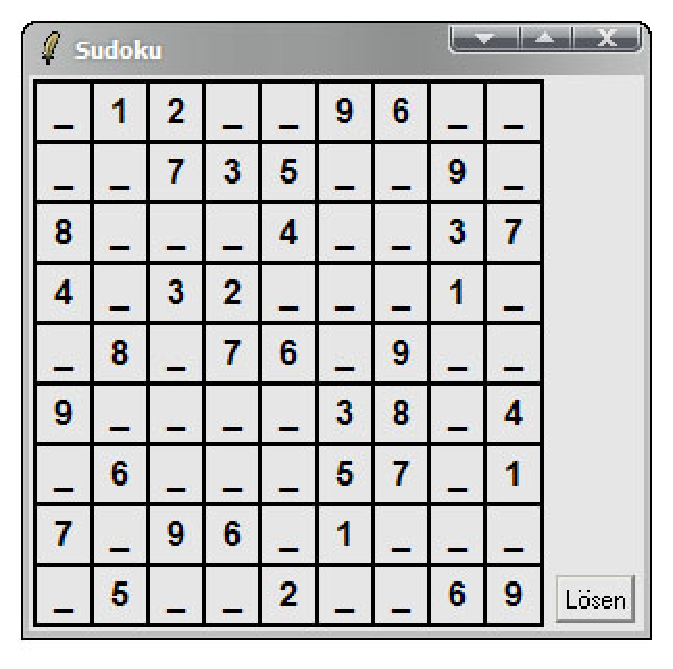
\includegraphics[width=0.4\textwidth]{../images/sudoku-unsolved}
   } 
   \subfloat[Gelöst]
   {
     \label{fig:sudoku-solved}
     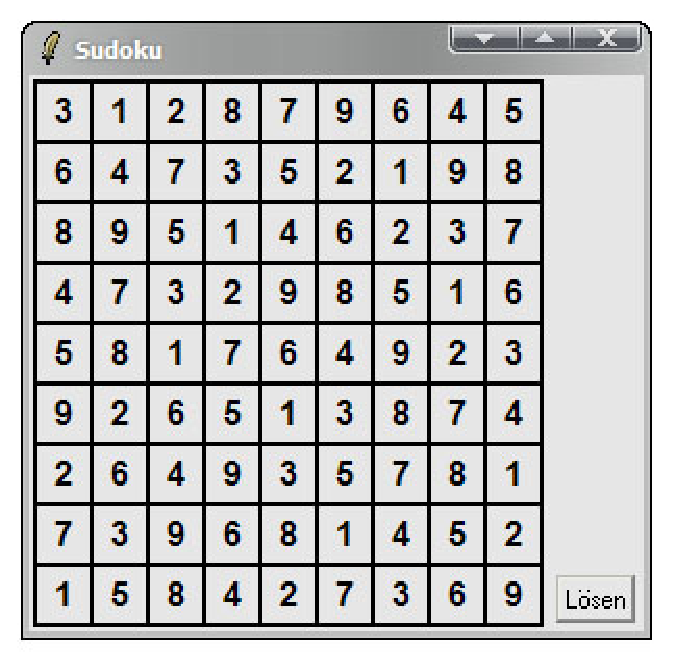
\includegraphics[width=0.4\textwidth]{../images/sudoku-solved}
   }
   \caption{Oberfläche des Sudoku-Lösers}
   \label{fig:sudoku-solver}
\end{figure}

\section{Funktionale Programmierung}
Die funktionale Programmierung fußt auf der Auswertung (mathematischer)
Ausdrücke. Funktionen verhalten sich hierbei - im Gegensatz zu anderen,
nicht-funktionalen Programmiersprachen - wie mathematische Funktionen. Dies hat
u.a. den Vorteil, dass Programme sich nun mit mathematischen Beweisverfahren
besser validieren lassen. Ein wichtiges Merkmal funktionaler Programme ist, dass
anstatt Schleifen und Zuweisungen mit Rekursion gearbeitet wird.

Oz unterstützt sowohl die sog. \textsl{eager evaluation} als auch
\textsl{lazy evaluation}. Eager evaluation (strikte Auswertung) bedeutet, dass
Argumente einer Funktion vor Ausführung der eigentlichen Funktion ausgewertet
werden. Im Gegensatz dazu werden Argumente bei der lazy evaluation erst bei
Bedarf ausgewertet, also dann, wenn deren Wert in einer Rechenoperation benötigt
wird.

Listing \ref{lst:mapEager} zeigt ein einfaches Beispiel für funktionale
Programmierung in Oz.

\lstinputlisting[label={lst:mapEager}, mathescape=false,
caption={Funktionales Programm mit eager evaluation}]{../mapEager.oz}

Der Funktion \texttt{Map} wird eine Liste sowie eine Funktion übergeben; die 
Funktion wird dann rekursiv auf alle Listenelemente angewandt. In Zeile 9 wird 
\texttt{Map} beispielhaft mit der Liste \texttt{[1 2 3 4]} und einer anonym 
definierten Funktion aufgerufen.

\section{Objektorientierte Programmierung}
Mit Einführung der Programmiersprache Smalltalk hat die objektorientierte 
Programmierung weite Verbreitung gefunden und ist heutzutage das in der 
Wirtschaft am häufigst eingesetzten Programmierparadigma. Objekte kapseln 
(veränderlichen) \textsl{Zustand} und \textsl{Verhalten}. Besonders in 
Anwendungen, die mit externen Systemen oder Anwendern interagieren eignen sich 
Objekte gut, um die Problemstellung imperativ zu formulieren und zu lösen 
\cite{KI-LP96}.

In Oz lassen sich Klassen mit Attributen und Methoden deklarieren und 
anschließend Objekte dieser Klassen erzeugen. Weiterhin kann der Anwender seine
Klassenhierarchie mit Mehrfachvererbung aufbauen. Listing \ref{lst:counter}
zeigt die Deklaration einer Klasse \texttt{Counter} sowie einige
Methodenaufrufe. 

\lstinputlisting[label={lst:counter}, mathescape=false,
caption={Deklaration einer Klasse und Erzeugen eines Objekts}]{../counter.oz}

In Zeile 16 wird ein Objekt der Klasse \texttt{Counter} erzeugt und der
Variablen \texttt{C} zugewiesen. Die Zeilen 17 und 18 zeigen Aufrufe der
Methoden \texttt{inc()} bzw. \texttt{browse()}.

\section{Logische Programmierung}
Mithilfe von logischen Programmiersprachen wie z.B. Prolog lassen sich Probleme
lösen, für die kein (effizienter) Algorithmus bekannt ist, man also nach der
Lösung \textsl{suchen} muss. Diese Art von Problem taucht bspw. in der
Künstlichen Intelligenz, der Sprachverarbeitung oder der Unternehmensforschung
(Operation Research) auf \cite[Tutorial of Oz,
Chapter 12]{url:mozart-documentation}.

Oz erweitert die Ideen von Prolog und setzt dabei nicht auf die von Prolog
bekannten Horn-Klauseln, sondern verwendet eine einfache Kompositions-Syntax
höherer Ordnung \cite{LogicProgr:2003}. 

Mithilfe der logischen Programmierung lassen sich aber nicht nur die genannten 
Suchprobleme lösen, sondern auch herkömmliche algorithmisch lösbare Probleme.
Listing \ref{lst:detAppend} zeigt zunächst ein \textsl{deterministisches}
Programm, d.h. es ist keine Suche nötig.

\lstinputlisting[label={lst:detAppend}, mathescape=false,
caption={Deterministisches logisches Programm}]{../detAppend.oz}

Die Funktion \texttt{Append} soll den übergebenen Parameter \texttt{Ys} an 
\texttt{Xs} anhängen und das Ergebnis zurückliefern. In Zeile 8 wird in dem 
beispielhaften Aufruf \texttt{X} an die Liste \texttt{[1 23 abc]} angehängt.

Im Gegensatz dazu wird bei der \textsl{nicht-deterministischen} Programmierung
davon ausgegangen, dass man nur durch Suche die bzw. alle Lösungen finden kann.
In Oz lässt sich so etwas mithilfe des \texttt{choice}-Statements realisieren,
wie Listing \ref{lst:nonDetAppend} zeigt.

\lstinputlisting[label={lst:nonDetAppend}, mathescape=false, 
caption={Nicht-deterministisches logisches Programm. Quelle: 
\cite{LogicProgr:2003}}]{../nonDetAppend.oz}

Hier wird zunächst wieder die Prozedur \texttt{Append} definiert, dieses mal
jedoch wird ein sog. \textsl{choice-point} festgelegt. Anschließend wird eine
weitere Prozedur \texttt{Anfrage} deklariert, welche die Suchanfrage beinhaltet
und das Ergebnis zurückliefert. Die eigentliche Suche wird über die Klasse
\texttt{Search} (s. auch Kapitel \ref{subsection:Search}) verwaltet. Über die
Methode \texttt{next()} (Zeile 21) lässt sich die jeweils nächste Lösung
ermitteln - auf diese Weise können sukzessive alle Lösungen bestimmt werden.
